\documentclass[11pt]{article}

\newcommand{\HWnum}{} 
\newcommand{\StudName}{Timothy Holmes} % author
\newcommand{\CourseNum}{474}           % course number
\newcommand{\Subject}{PHY}

\usepackage{graphicx, amsmath, amssymb,fancyhdr}
\addtolength{\textwidth}{1.5in}
\addtolength{\oddsidemargin}{-2cm}
\addtolength{\evensidemargin}{-2cm}
\addtolength{\textheight}{1.6in}
\addtolength{\topmargin}{-0.7in}
\addtolength{\headsep}{-0.1in}
%\addtolength{\footskip}{-0.2in}
\pagestyle{fancy}
\cfoot{}
\lhead{\textbf{\Subject ~ \CourseNum~--- Homework~\HWnum}}
\rhead{\textbf{\StudName:~Page~\thepage}}

\addtolength{\parskip}{\baselineskip} % skips a line between paragraphs
\parindent 0in                        % no indent at start of paragraph

\newcommand{\dd}{\textrm{d}}
\usepackage{braket}
\usepackage{lipsum, babel}
\usepackage{blindtext}
\usepackage{graphicx}% Include figure files
\usepackage{dcolumn}% Align table columns on decimal point
\usepackage{bm}% bold math
\usepackage{listings}
\usepackage{listing}
\usepackage{supertabular}



\usepackage{color} %red, green, blue, yellow, cyan, magenta, black, white
\definecolor{mygreen}{RGB}{28,172,0} % color values Red, Green, Blue
\definecolor{mylilas}{RGB}{170,55,241}




\lstset{language=Python,%
    %basicstyle=\color{red},
    breaklines=true,%
    morekeywords={matlab2tikz},
    keywordstyle=\color{blue},%
    morekeywords=[2]{1}, keywordstyle=[2]{\color{black}},
    identifierstyle=\color{black},%
    stringstyle=\color{mylilas},
    commentstyle=\color{mygreen},%
    showstringspaces=false,%without this there will be a symbol in the places where there is a space
    numbers=left,%
    numberstyle={\tiny \color{black}},% size of the numbers
    numbersep=9pt, % this defines how far the numbers are from the text
    emph=[1]{for,end,break},emphstyle=[1]\color{red}, %some words to emphasise
    %emph=[2]{word1,word2}, emphstyle=[2]{style},    
}

\begin{document}
% -------------------------- BOD -------------------------- 

\title{Homework {\HWnum}}
\author{Timothy Holmes \\ \Subject ~ \CourseNum ~ Stellar Astrophysics}

\maketitle

\section*{Problem 1}

\subsection*{(a)}

We can find 
$$
\frac{10 \% \; \text{mass converted to He} \cdot M_{\odot}}{(4 \cdot (m_{p}))} = \frac{0.10 * 2.18 \times 10^{30} \; kg}{(4 \cdot (1.67 \times 10^{-27} \; kg))} = 3.26 \times 10^{55} \; \text{reactions}
$$
where $2.18 \times 10^{30} \; kg = 1.1 \; M_{\odot}$.

\subsection*{(b)}

We can find how much energy Centauri A produces in its Main Sequence lifetime. We know that the energy released when four hydrogen nuclei are fused into one helium nucleus in the pp-chain, 26.7 MeV of energy is release. In order to calculate this we can take the number of helium nuclei obtained in part (a) and multiply it by energy released in the PP-chain to get
$$
E = 3.26 \times 10^{55}  \; \text{reactions} \cdot 26.7 \frac{MeV}{ \; \text{reactions}} = 8.71 \times 10^{56} MeV = 1.40 \times 10^{44} J.
$$

\subsection*{(c)}

The equation for luminosity is gave by $L = E/t$. In part (b) we found the value for $E$. Therefore, we can solve for time by 

$$
t = \frac{E}{L} = \frac{1.40 \times 10^{44} J}{5.74 \times 10^{26} \; W } = 2.43 \times 10^{17} s = 7.73 Gyr
$$
where $5.74 \times 10^{26} \; W = 1.5 \; L_{\odot}$.

\clearpage

\section*{Problem 2}
The kinetic energy of protons at which quantum mechanical tunneling has a significant probability is
$$
E \approx \Bigg(\frac{e^{2}}{4 \pi \epsilon_{0}}\Bigg)^{2} \frac{2m_{p}}{h^{2}}
$$

\subsection*{(a)}

For $H$, 
$$
E \approx \Bigg(\frac{e^{2}}{4 \pi \epsilon_{0}}\Bigg)^{2} \frac{2m_{p}}{h^{2}} 
$$
For $He$, 
$$
E \approx \Bigg(\frac{2 \cdot e^{2}}{4 \pi \epsilon_{0}}\Bigg)^{2} \frac{4 \cdot 2 \; m_{p}}{h^{2}}
$$

\subsection*{(b)}

The temperature for hydrogen fusion and helium fusion can be found using 
$$
E = (3/2)kT
$$
we can solve for temperature and the equation becomes
$$
T = \frac{2E}{3k}.
$$
The energy for hydrogen fusion can be calculated by
$$
E_{H} = \Bigg(\frac{(1.60 \times 10^{-19} \; C)^{2}}{4 \pi (8.85 \times 10^{-12} \; F \; m^{-1}}\Bigg)^{2} \frac{2 \; (1.67 \times 10^{-27} \; kg)}{(6.63 \times 10^{-34} \; m^{2} \; kg \; s^{-1})^{2}} = 4.02 \times 10^{-16} \; J
$$
Since the energy for helium is 64 times higher than hydrogen, then we can find the energy for helium by
$$
E_{He} = 64 \cdot E_{h} = 64 \cdot (4.02 \times 10^{-16} \; J) = 2.56 \times 10^{-14} \; J
$$
With these two values now calculated, the temperature can now be computed, the temperature for $H$ is 
$$
T = \frac{2(4.02 \times 10^{-16} \; J)}{3(1.38 \times 10^{-23} \; J \; K^{-1})} = 19 \times 10^{6} \; K.
$$
and the temperature for $He$ is
$$
T = \frac{2( 2.56 \times 10^{-14} \; J)}{3(1.38 \times 10^{-23} \; J \; K^{-1})} = 1237 \times 10^{6} \; K.
$$

\clearpage

\section*{Problem 3}

\subsection*{(a)}

\begin{figure}[h!]
    \centering
    {{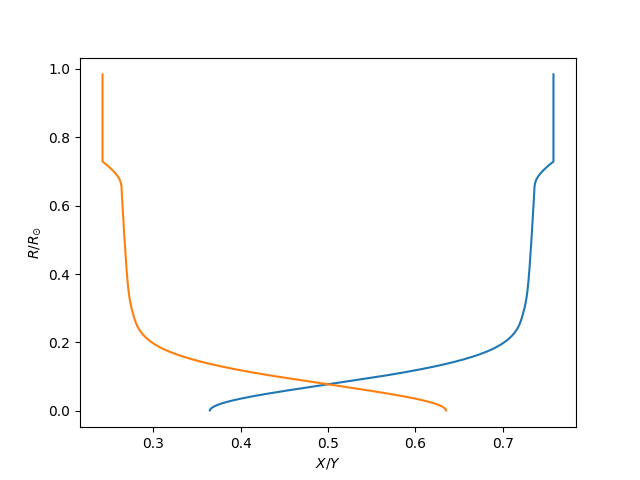
\includegraphics[width=15cm]{Figure_1.png} }}%
    \caption{}%
    \label{fig:example}%
\end{figure}

\subsection*{(b)}

What we see in the plot above is the yellow line is the hydrogen mass fraction while the blue line is the helium mass fraction. Just like plots we see in E&M or quantum mechanics with transmission and reelection coefficients, when one increases the other has to decrease. The same is true in the case of mass fractions. While hydrogen will eventually fuse into helium, the amount of hydrogen will have to decrease while the amount of helium will increase as time increases. This is what we are seeing here when comparing it to the radius as the radius will change over time and will help with the process.

\newpage

\subsection*{(c)}

\begin{figure}[h!]
    \centering
    {{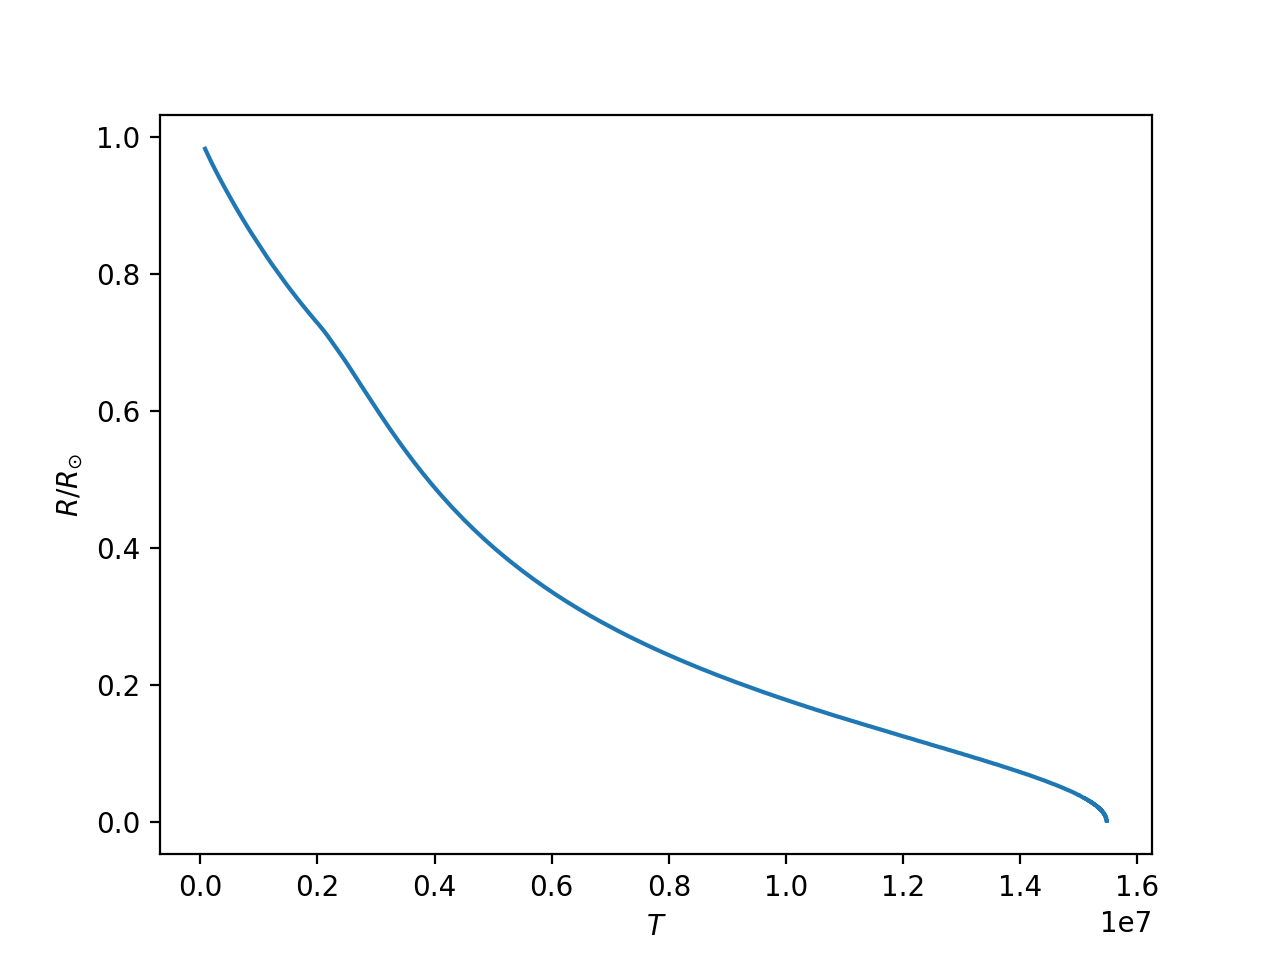
\includegraphics[width=15cm]{Figure_2.png} }}%
    \caption{}%
    \label{fig:example}%
\end{figure}

\newpage

\subsection*{(d)}

\begin{figure}[h!]
    \centering
    {{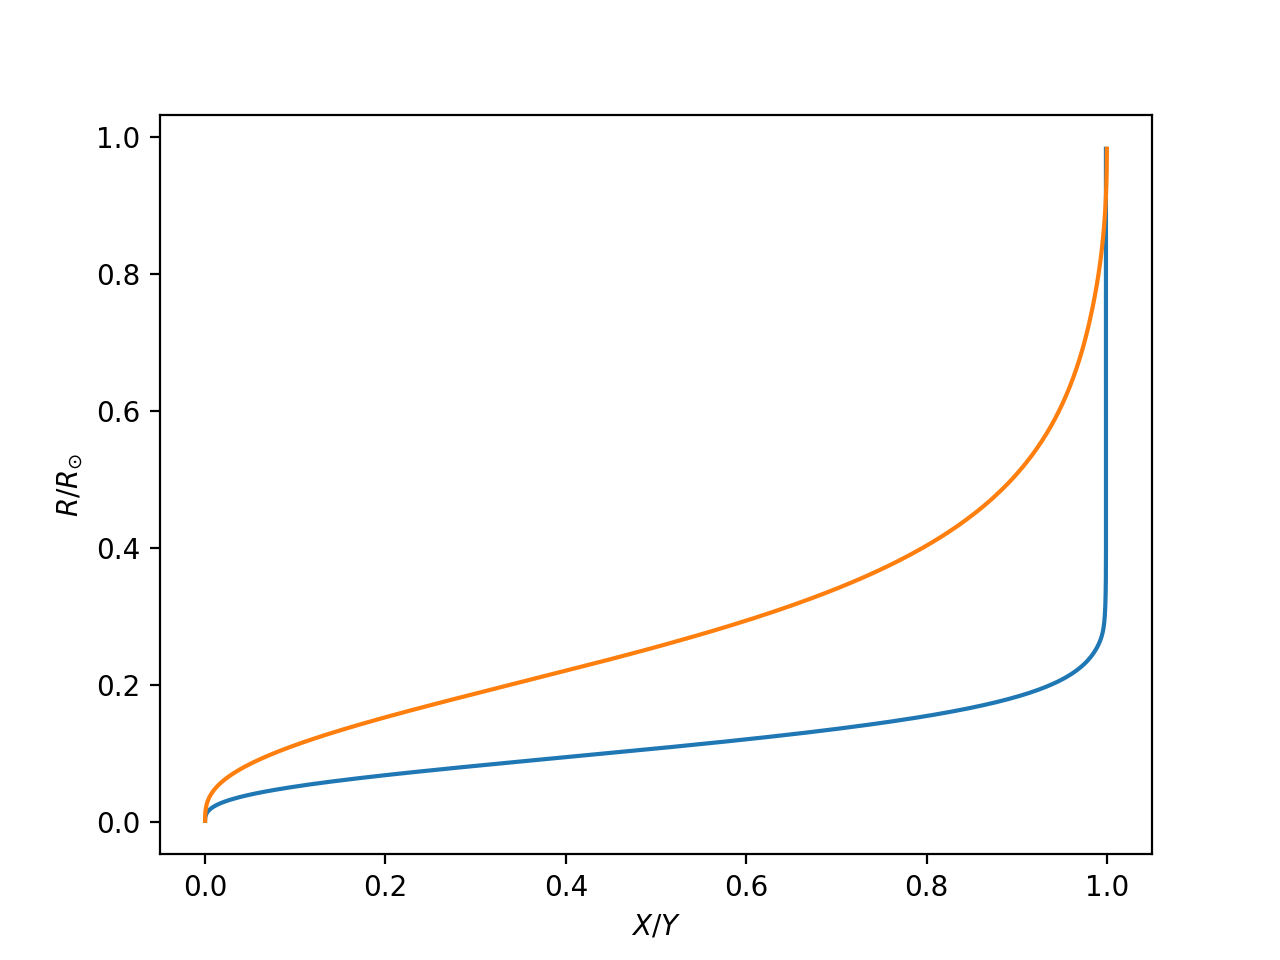
\includegraphics[width=15cm]{Figure_3.png} }}%
    \caption{}
    \label{fig:example}%
\end{figure}

\clearpage

\section*{Problem 4}

Reimer's law for the mass loss rate on the Asymptotic Giant Branch is gave by
$$
\frac{dM}{dt} = -\frac{c \eta LR}{M}
$$
where $L$ is the luminosity, $R$ is the radius, $c = 4 \times 10^{-13}$, $\eta ~ 1$, and $M$ is the mass of the AGB star in solar units, and $dM/dt$ is the mass loss rate of the AGB star in $M_{\odot} \; yr^{-1}$. To integrate this equation, we need to rearrange thee terms such that
\begin{align*}
    \int_{M_{0}}^{M} M \; dM &= - c \eta L R \int_{0}^{t} dt 
\end{align*}
Evaluating this integral we get 
\begin{align*}
    \Bigg[ \frac{M^{2}}{2} \Bigg]_{M_{0}}^{M} &= - c \eta L R \big[ t \big]_{0}^{t} \\ \\
    \Bigg[ \frac{M^{2}}{2} - \frac{M_{0}^{2}}{2} \Bigg] &= - c \eta L R \big[ t - 0 \big] \\ \\
    \frac{M^{2} - M_{0}^{2}}{2} &= - c \eta L R t \\ \\
    M^{2} - M_{0}^{2} &= - 2 c \eta L R t \\ \\
    M^{2} &=  M_{0}^{2} - 2 c \eta L R t 
\end{align*}
Thus, we get the final equation
$$
M(t) &=  \sqrt{M_{0}^{2} - 8 \times 10^{-13} L R t} \\ 
$$

\clearpage

\section*{Appendix}

\subsection*{Homework 5 Program}
\lstinputlisting{homework_5.py}

\clearpage


% -------------------------- EOD -------------------------- 
\end{document}